\documentclass{article}

\usepackage[utf8]{inputenc}
\usepackage[french]{babel}

\usepackage{lmodern}
\usepackage{graphicx}
\usepackage{hyperref}
\usepackage{graphicx}
\usepackage{natbib}
\graphicspath{ {./res/} }

\author{
    Valentin Jonquière,
    Mathilde Chollon,
    Denis Demirci,
    Iwen Jomaa,
    Jonathan Landry
}

\title{Rapport Préliminaire projet de programmation, Échecs en Java}

\begin{document}

\maketitle

\pagebreak

\tableofcontents

\pagebreak

\section{Contexte du sujet}
\subsection{Sujet choisi}
Nous avons choisi le sujet '\textit{les échecs}' car nous avons abordé ce jeu
plusieurs fois et dans différentes disciplines. Nous avions par exemple illustré un 
cours d'intelligence artificielle au semestre dernier avec celui-ci, mais 
également un cours d'algorithmie par le passé. Nous avons donc quelques connaissances 
utiles pour réaliser certains des besoins et qui nous permettent plus généralement de ne pas
découvrir entièrement le sujet.

\subsection{Existant}
Les échecs étant un jeu universel, ils ont été étudiés et un grand nombre de papiers scientifiques
sont disponibles. Ceux-ci nous seront très utiles tout au long du projet, car ils concernent des
besoins différents. Tout d'abord une grande partie des papiers que nous allons utiliser sont en rapport
avec la partie intelligence artificielle du développement. C'est pour cela que nous avons par exemple
choisi de nous baser sur l'article `Programming a computer for playing chess' \cite{Shannon1950}, 
puisqu'il possède une partie consacrée à la construction d'heuristiques efficace pour les échecs.
Nous avons également basé nos recherches sur la thèse `Using Monte Carlo Tree Search to play chess' \cite{Kral2021}
de Jakub Král sur l'utlisation de différents algorithmes au service des échecs, tels que AlphaBeta ou
Monte Carlo Tree Seach  \cite{ZobristHashing}

\subsection{Langage de programmation choisi}
Avec ce sujet, nous avions 3 choix de langage possibles :
\begin{itemize}
    \item Le langage C
    \item Le Java
    \item Le Python
\end{itemize}
Même si nous avons dû faire un choix rapidement, nous avons d'abord développé les
avantages et inconvenants de chacun de ces langages. De plus, nous nous étions mis
d'accord sur quelques besoins essentiels auquel certains des langages ci-dessus 
n'aurait pas (ou difficilement) pu répondre.
Tout d'abord nous souhaitions pouvoir développer notre logiciel sous forme de modules
complémentaires, pour plusieurs raisons.
\begin{itemize}
    \item Nous avons convenu de baser les 8 semaines de code en se concentrant sur 
    des blocs de 2 semaines avec, pour chaque bloc, une liste de 2 ou 3 modules à développer.
    \item Isoler les bugs dans chaque module afin d'avoir moins de problèmes lors de la fusion
    des modules.
    \item Facilité de maintien. Avec 8 semaines de code, il est essentiel que nous possédions
    un logiciel organisé afin de ne pas avoir à `fouiller' dans le code écrit la première semaine
    lors de la finalisation du projet.
    \item Utilisation de la programmation objet. Même s'il n'y a pas d'extension de prévue,
    ce paradigme est le plus simple et adopté lors du développement d'un jeu.
\end{itemize}

\subsubsection{Langage C}
La première option qui nous était proposée été le langage C. Le projet contenant des besoins posant
des contraintes de performances (cf. besoin), ce langage a donc semblé être une bonne idée, car il est
de loin celui permettant d'obtenir un logiciel performant. Cependant, celui-ci ne proposant pas de 
possibilité de développement objet, nous aurions dû faire une grosse concession dès le choix du langage.
De plus, la gestion de la mémoire étant à la charge du développeur, nous aurions pu rester bloqué un temps
précieux sur un pointeur mal alloué. Cette gestion de la mémoire apporte également le problème des fuites
mémoire qui demandent, elle aussi, parfois beaucoup de travail pour être résolues.

\subsubsection{Python}
Nous pouvions également utiliser \textit{Python} pour réaliser ce projet. Cependant, le fait que ce langage
soit non typé a vite écarté ce choix. En effet, les types étant vérifiés directement à l'exécution, il est
beaucoup plus dangereux d'avoir une ligne non couverte par un test (il faut donc un coverage maximal). Il y
a donc le danger de laisser des erreurs de typages qui ne sont découverte uniquement lorsqu’une partie du code
est exécutée après la livraison du code.

\subsubsection{Java}
Nous avons donc fini par opter pour \textit{Java}. En effet, il permet tout comme \textit{Python} de faire
de la programmation objet, mais avec plus de rigueur. Étant conçu pour le développement objet, il y a moins
de chance de mélanger plusieurs paradigmes et de se retrouver avec un code mi-objet/mi-impératif. De plus,
le typage statique permet d'avoir une meilleure stabilité grâce à la détection des erreurs de types à la 
compilation et permet également d'avoir un code plus prévisible. Enfin, les plus projets réalisés en licence
et en master étant souvent des projets java, tous les membres du groupe connaissent ce langage ainsi que ses
outils et environnements de développement. Cela permettra de gagner du temps lors de la mise en place du projet. 

\section{Explication du sujet}
\subsection{Structures de données}
\subsubsection{Historique des coups}
Le groupe s'est posé la question de quelles structures de donneés utiliser pour stocker l'historique des coups d'une
partie. Il a fallu prendre en compte plusieurs facteurs, notamment la performance, la ou les difficultés d'implémentation,
la compatibilité avec les bitboards pour représenter le plateau de jeu, ainsi que les ajouts potentiels de fonctionnalités.
\\La première idée fut une pile. En effet, cette structure est très simple d'utilisation et parfaitement adaptée pour stocker
des coups, tout en ayant la possibilité d'en enlever et d'en rajouter. La complexité en temps et en espace est en O(n) si n 
correspond au nombre de coups de la partie. Pour revenir au tout début de la partie, c'est-à-dire avec les pièces positionnées
sur leurs cases initiales, il suffit de dépiler les n coups stackés en les empiler dans une seconde pile qui s'occupera de sauvegarder
ces coups pour pouvoir revenir au dernire coup joué avant d'avoir repris tous les coups. Ainsi, en utilisant la pile comme structure 
de données, on garde n coups en mémoire, et revenir à une certaine position de la partie est linéaire en fonction de ce nombre de coups.
Avec une interface graphique, on pourrait cliquer sur un certain coup pour savoir combien de coups dépiler, car un coup peut arriver
plusieurs fois dans une partie donc sa représentation ne suffit pas.\\
Cela se présenterait comme ceci:\\
%\begin{figure}[h]
%    \caption{Exemple historique de coups}
%    \centering
%    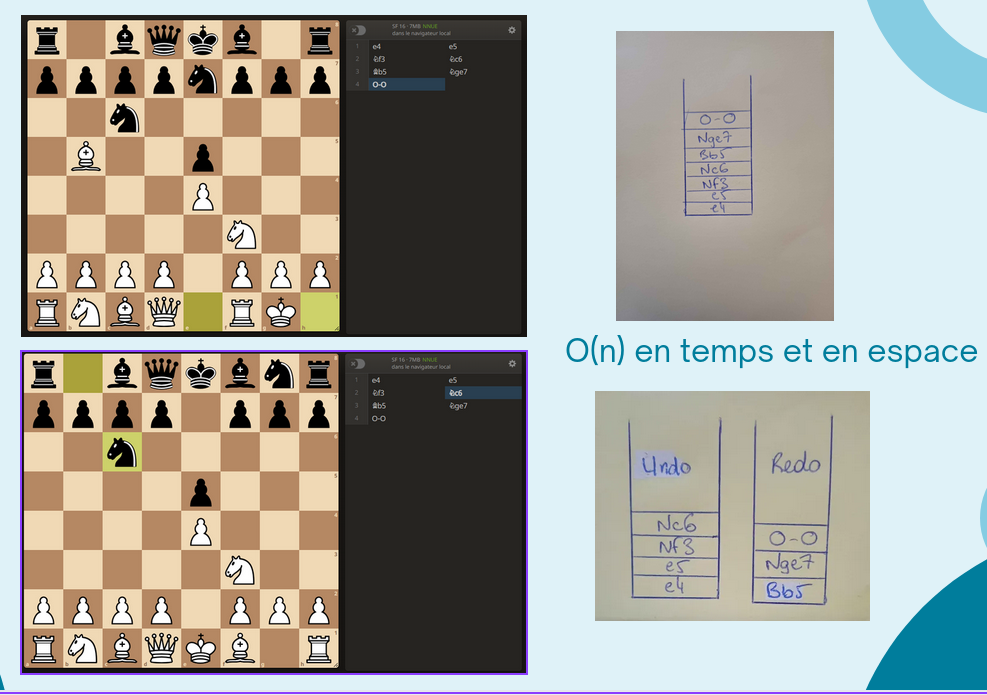
\includegraphics[width=\textwidth,height=\textheight,keepaspectratio]{pile-historique-coups.png}
%\end{figure}

S'il n'y a pas de fonctionnalité de game review

\section{Besoins visés}
\subsection{Quels besoins ?}
Dans le sujet donné, il y avait une liste de 60 besoins.
Nous avons pris la décision ambitieuse de répondre à tous ces besoins. C'est un travail conséquent,
mais avec une équipe de 5 personnes, codant pendant huit semaines,
nous pensons que cet objectif est atteignable.

Nous avons tout de même classé ces besoins par ordre de priorité (voir \nameref{agenda}), afin de garantir
la jouabilité projet même si nous n'arrivons pas à tout implémenter à temps.
Nous voulons rendre un jeu cohérent et fonctionnel avec des modules entièrement
terminés (même s'il en manque) plutôt qu'un projet avec des règles manquantes,
une intelligence artificielle bâclée et une interface graphique peu fonctionnelle.

\subsection{Dépendances entre les besoins}
\subsubsection{Gestion des options}
La première dépendance que nous avons concerne la gestion des options (Figure \ref{fig:needs_options}).

\begin{figure}[h]
    \caption{Besoins concernant la gestion d'options}
    \centering
    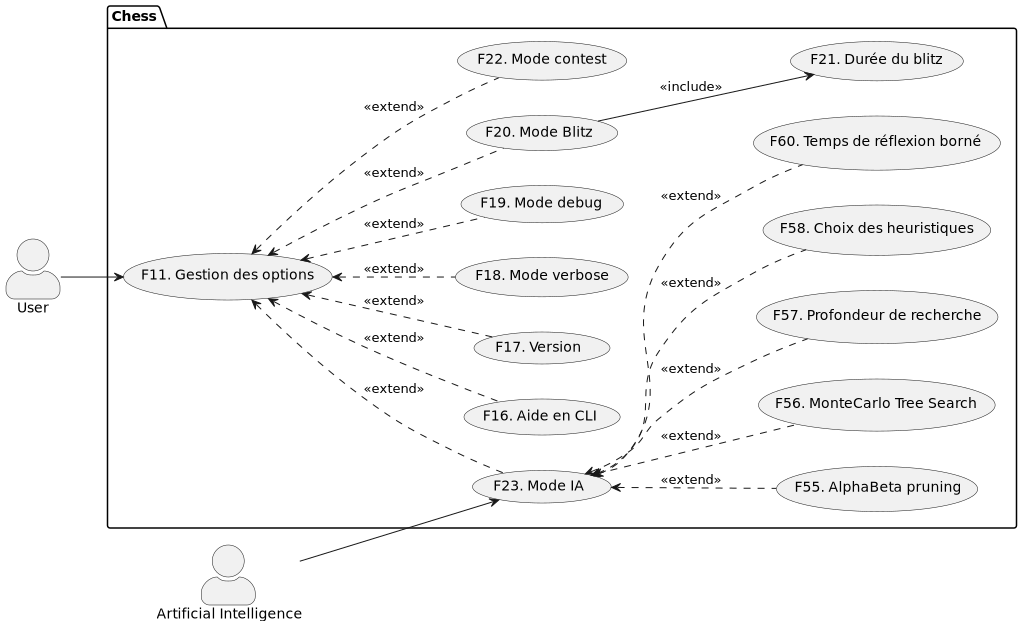
\includegraphics[width=\textwidth,height=\textheight,keepaspectratio]{needs_options}
    \label{fig:needs_options}
\end{figure}

L'implémentation de la \textit{gestion des options }permettra de rajouter de nombreuses fonctionnalités.
En effet, ceci nous permettra d'implémenter le Mode contest, la version du jeu ou l'aide en ligne de commande. Nous pourrons également gérer les messages affichés grâce au mode verbose ou au mode debug.
Lorsque cela sera implémenté, l'utilisateur aura également le choix entre afficher le jeu en ligne de commande ou avec une interface graphique.
Le mode Blitz inclura le besoin Durée du blitz afin de paramétrer ce mode.
Le mode IA, qui a besoin de la gestion des options, possède quant à lui de nombreuses extensions. En effet, nous pourrons paramétrer
notre intelligence artificielle grâce à d'autres options, que nous verrons cela plus en détail à la section \ref{IA}.


\subsubsection{Sauvegarde de l'historique}
La gestion de l'historique est un besoin indispensable pour notre jeu (Figure \ref{fig:needs_files}).
Beaucoup de besoins dépendent de cette fonctionnalité.
\begin{figure}[h]
    \caption{Besoins concernant la sauvegarde de l'historique}
    \centering
    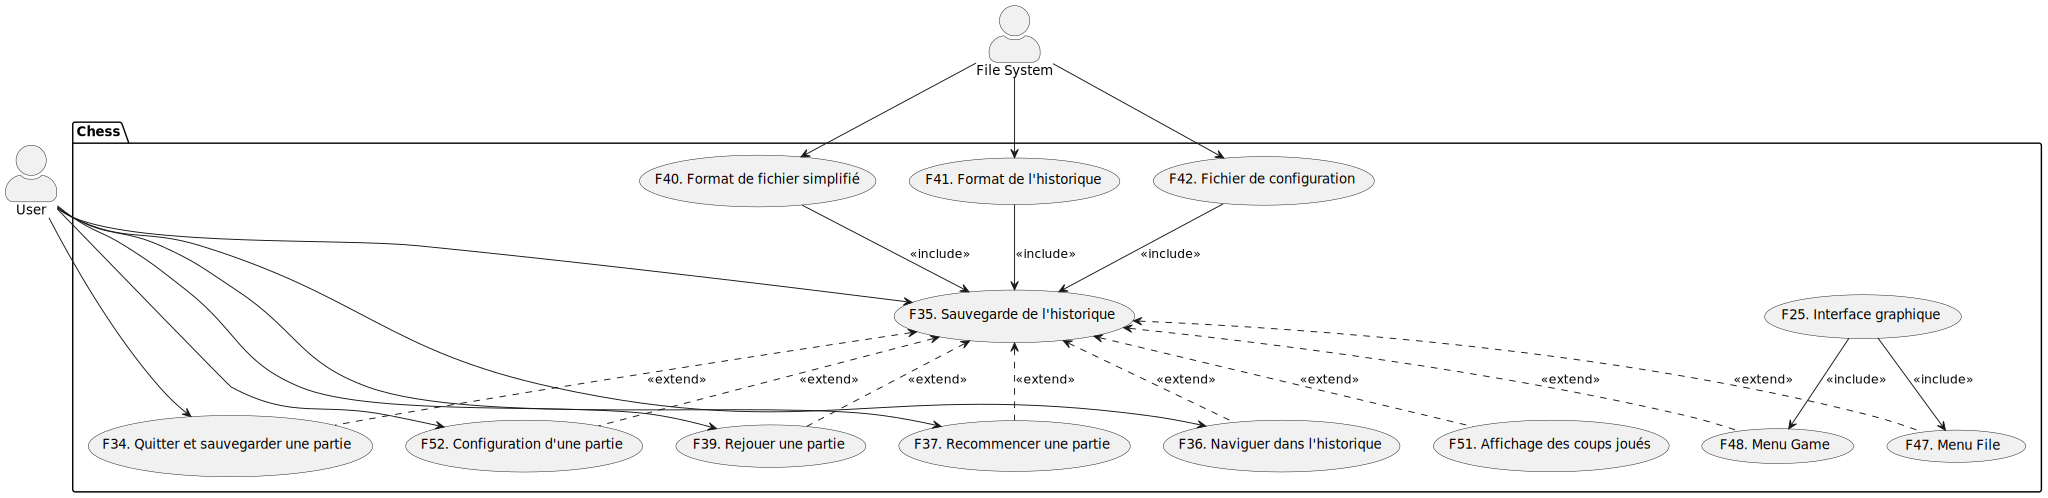
\includegraphics[width=\textwidth,height=\textheight,keepaspectratio]{needs_files}
    \label{fig:needs_files}
\end{figure}

Avant de pouvoir implémenter la gestion de l'historique, il faudra d'abord choisir les formats de fichiers.
Pour cela, il faudra remplir les besoins suivants: \textit{Format de fichier simplifié}, \textit{Format de l'historique} et \textit{Fichier de Configuration}.
Une fois ces besoins implémentés, la sauvegarde de l'historique sera donc possible.
Des besoins utiles au bon déroulement du jeu en dépendent. Grâce à cela, l'utilisateur pourra sauvegarder
sa partie, rejouer ou recommencer une partie. Il pourra également configurer sa partie en modifiant les données du fichier de configuration.
Cela permettrait aussi d'afficher les coups précédemment joués, et même de remonter dans l'historique pour annuler un coup et revenir en arrière.
Certains menus de l'interface graphique permettront également de gérer ces fichiers de sauvegarde et de configuration (voir figure \ref{fig:needs_gui}).

\subsubsection{Intelligence artificielle}
\label{IA}
L'implémentation d'une intelligence artificielle est un autre besoin central du jeu. En effet, cela pourra
permettre à l'utilisateur de jouer contre une machine. Cela pourrait également permettre de donner des
indications sur les meilleurs coups à jouer pour le joueur.

\begin{figure}[h]
    \caption{Besoins concernant l'intelligence artificielle}
    \centering
    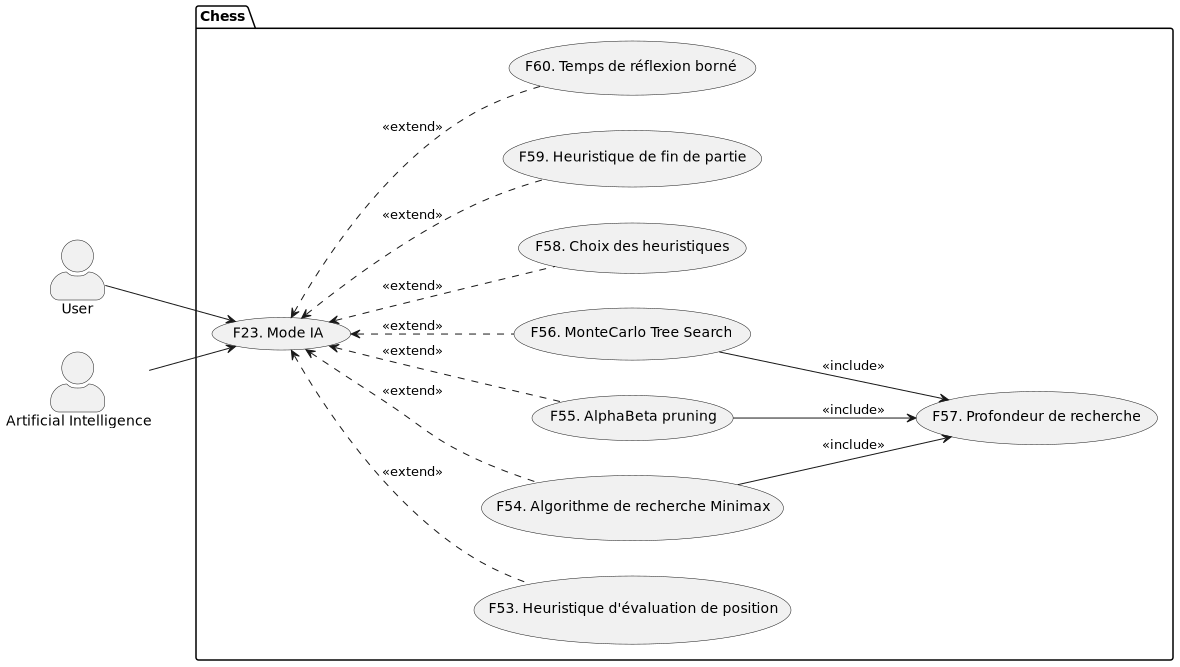
\includegraphics[width=\textwidth,height=\textheight,keepaspectratio]{needs_ai}
    \label{fig:needs_ai}
\end{figure}

Comme affiché Figure \ref{fig:needs_ai}, nous pouvons voir que de nombreux besoins
concernent l'intelligence artificielle.
La plupart des besoins affichés sont également présent dans la Figure \ref{fig:needs_options}, car ils sont paramétrables
en ligne de commande.
Le mode IA contient différentes fonctionnalités concernant les heuristiques. Nous devons implémenter différentes \textit{heuristiques}
d'évaluation de position, mais également au moins une heuristique de fin de partie. Ces heuristiques permettront "d'aider" le joueur IA
à jouer. Ces heuristiques pourront être utilisées avec l'\textit{algorithme de recherche Minimax} mais également lors de l'\textit{AlphaBeta pruning} 
et le \textit{Monte Carlo Tree Search}. Ces algorithmes dépendent tous de l'option \textit{Profondeur de recherche}. En effet, le jeu des échecs est bien 
trop complexe pour simuler une partie entière, et nous devons nous limiter à une certaine profondeur de recherche (nombre de coups à jouer puis analyser).
Borner le temps de "réflexion" de l'IA est aussi un moyen de limiter les calculs de ces algorithmes. Cela pourrait permettre à l'utilisateur de jouer une partie contre
un joueur IA plus ou moins efficace ou d'attendre plus ou moins longtemps entre ses tours.
\subsubsection{Interface graphique}
Les derniers besoins que nous avons rassemblé sont ceux concernant l'interface graphique (Figure \ref{fig:needs_gui}).
\begin{figure}[h]
    \caption{Besoins concernant l'interface graphique}
    \centering
    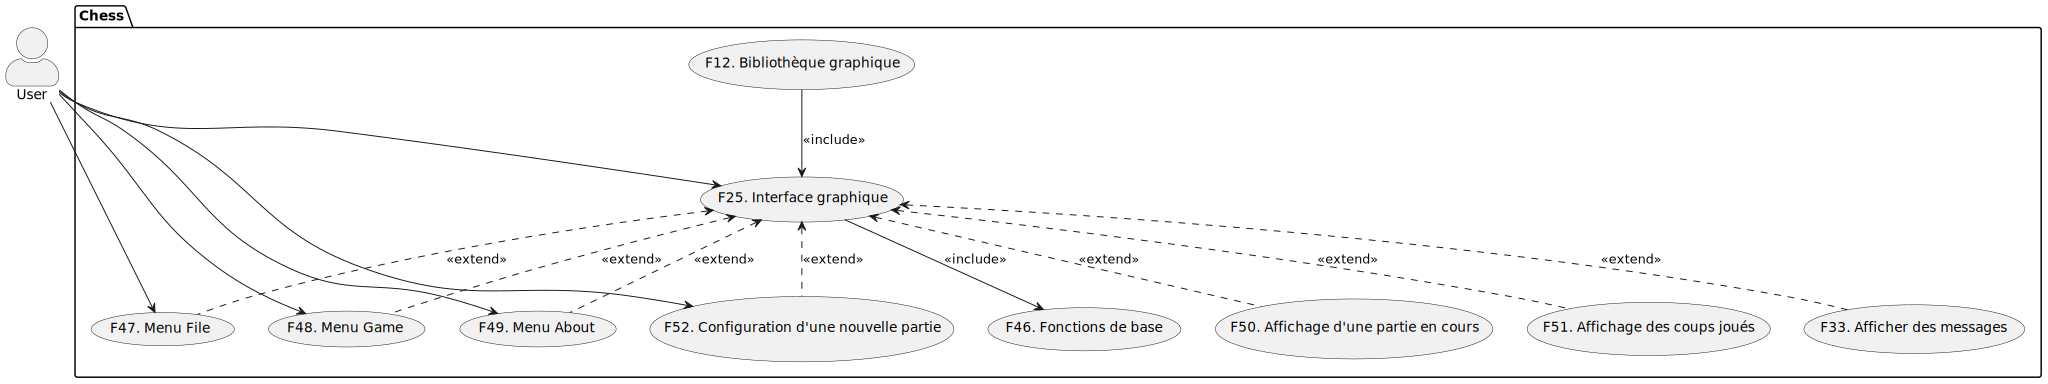
\includegraphics[width=\textwidth,height=\textheight,keepaspectratio]{needs_gui}
    \label{fig:needs_gui}
\end{figure}

L'interface graphique dépend de la \textit{bibliothèque graphique} choisie, ici elle est imposée, il s'agit de \textit{JavaFX}.
L'utilisateur peut choisir de l'utiliser grâce aux options en ligne de commande (Figure \ref{fig:needs_options}).
Elle doit permettre d'utiliser les fonctions de base que nous avons implémenté pour le jeu en ligne de commande. Nous devons 
pouvoir afficher la partie en cours, les coups joués, ainsi que des messages selon le mode utilisé (Verbose ou Debug, voir figure \ref{fig:needs_options}).
L'utilisateur doit également pouvoir utiliser différents menus afin de pouvoir paramétrer ou sauvegarder sa partie (voir figure \ref{fig:needs_files}) ou obtenir des informations sur le jeu.

\section{Agenda prévisionnel}
\label{agenda}

Nous avons décidé de séparer le temps de programmation en quatre parties. Les trois premières seront rythmées besoin par besoin, et la dernière quant à elle sera dédiée à la finalisation du projet et la préparation d'un livrable.
Une partie des besoins sera également suivie tout au long du projet afin de maintenir une base cohérente.

\subsection{Tout au long du projet}

Gestion des aspects fondamentaux et comme le style de codage, les tests, les performances, et la documentation pour garantir la cohérence et la qualité globale du code.

\begin{itemize}
    \item F1. Langage de programmation
    \item F2. Style de codage
    \item F3. Langue par défaut dans le code
    \item F4. Système cible
    \item F5. Documentation
    \item F6. Tests
    \item F10. Frameworks de tests
    \item F7. Bugs
    \item F8. Performances
    \item F9. Build-system
    \item F14. Nom de l’exécutable principal
    \item F15. Usage général
\end{itemize}

\subsection{Semaines 0-2}

Mise en place des fonctionnalités essentielles pour le jeu en ligne de commande, telles que la gestion des options CLI, les règles de jeu, et l'affichage de l'échiquier.

\begin{itemize}
    \item \textbf{Options CLI :}
    \begin{itemize}
        \item F11. Gestion des options
        \item F16. Aide en ligne de commande
        \item F17. Version
        \item F18. Mode verbose
        \item F19. Mode debug
        \item F13. Internationalisation
    \end{itemize}
    \item \textbf{Gestion du jeu :}
    \begin{itemize}
        \item F43. Plateau de jeu
        \item F44. Module bitboard
        \item F45. État du jeu
    \end{itemize}
    \item \textbf{Règles :}
    \begin{itemize}
        \item F29. Prise en passant
        \item F30. Roque
        \item F31. Promotion du pion
        \item F38. Fin de partie
    \end{itemize}
    \item \textbf{Jeu CLI :}
    \begin{itemize}
        \item F24. Interface en ligne de commande
        \item F26. Affichage de l’échiquier
        \item F27. Notation des coups
        \item F28. Représentation de l’historique
        \item F33. Affichage des messages
    \end{itemize}
\end{itemize}

\subsection{Semaines 2-4}

Développement de l'IA, avec des algorithmes comme Minimax et Monte Carlo, et ajout de fonctionnalités avancées comme la sauvegarde, la navigation dans l'historique, et le fichier de configuration.

\begin{itemize}
    \item \textbf{IA :}
    \begin{itemize}
        \item F23. Mode IA
        \item F53. Heuristique d’évaluation de position
        \item F54. Algorithme de recherche Minimax
        \item F55. $\alpha\beta$-pruning
        \item F56. Monte Carlo Tree Search
        \item F57. Profondeur de recherche
        \item F59. Heuristique de fin de partie
        \item F60. Temps de réflexion borné
    \end{itemize}
    \item \textbf{Fonctionnalités :}
    \begin{itemize}
        \item F32. Abandon
        \item F34. Quitter et sauvegarde une partie
        \item F35. Sauvegarde de l’historique
        \item F36. Naviguer dans l’historique
        \item F37. Recommencer une partie
        \item F40. Format de fichier simplifié
        \item F41. Format de l’historique
        \item F42. Fichier de configuration
    \end{itemize}
\end{itemize}

\subsection{Semaines 4-6}

Création de l'interface graphique et finalisation des fonctionnalités utilisateurs, incluant les menus interactifs, la gestion des parties, et les modes spéciaux comme le mode blitz et contest.

\begin{itemize}
    \item \textbf{Interface graphique :}
    \begin{itemize}
        \item F12. Bibliothèque graphique
        \item F25. Interface graphique
        \item F46. Fonctions de base
        \item F47. Menu ’File’
        \item F48. Menu ’Game’
        \item F49. Menu ’About’
        \item F50. Affichage d’une partie en cours
        \item F51. Affichage des coups joués
        \item F52. Configuration d’une nouvelle partie
    \end{itemize}
    \item \textbf{Fonctionnalités :}
    \begin{itemize}
        \item F20. Mode blitz
        \item F21. Durée du blitz
        \item F22. Mode contest
        \item F39. Rejouer une partie
        \item F58. Choix des heuristiques
    \end{itemize}
\end{itemize}

\section{Architecture visée pour le projet}

\section{Spécifications étendues}

\section{Bibliographie}
\bibliographystyle{plain}
\bibliography{references}
\end{document}